% !TEX root = ../main.tex
\section{Psychology and Human Factors}\label{sec:humanfactors}

	In many years, the field of psychology have been important in order to understand how humans interpret and remember information. Psychology studies have recognized that the human brain have a superior memory for recognizing and recalling visual information rather than recognizing and recalling verbal or textual information \cite{DeAngeli}. To be able to go beond the technical part of security, this chapter will include related work on passwords focusing on psychology and the human aspects. Combining research from two different diciplines, computer security and psychology, will give a deeper understnading of passwords at a different level. 

		\begin{wrapfigure}{r}{0.4\textwidth}
      \vspace{-10pt}
      \begin{center}
        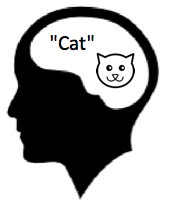
\includegraphics[scale=0.5]{pics/review/dualCoding.png}
      \end{center}
      \vspace{-10pt}
      \caption{Dual-Coding Theory}
      \vspace{-10pt}
      \label{fig:dualcoding}
    \end{wrapfigure}

	One known theory from the world of psychology is the ``dual-coding theory'' \cite{Biddle}. The theory suggests that verbal and non-verbal memory are processed and represented differently in human's mind. Text are verbal information that is represented symbolically, in contrast to non-verbal information like images that are mentally represented in a way that perceived concepts are assigned to a perceived meaning of what is directly observed. Both verbal and non-verbal information can be used when recalling information. For example, say a person have received stimulus of the concept ``cat'', both the image of a cat as well as the word ``cat'' (Figure~\ref{fig:dualcoding}). When a person is asked to recall the concept ``cat'', a person can retrieve the image or the word individually, or both simultaneously. If the word ``cat'' is remembered, the picture of the cat is not lost and can still be retrieved at a later point in time. The ability to code a stimulus in two different ways can increase humans ability to remember, in contrast to only code the stimulus in one way. In the background theory there are described three various categories of graphical passwords according to the memory task involved in remembering and entering the password, e.g. recall, recognition and cued recall.

	When it comes to humans and visual interpretation, studies support the idea that people recall symmetric images better than asymmetric images \cite{Attneave, French}. A particular interesting observation is that mirror symmetry carries a special status I the human memory \cite{Wagemans1}. An understanding of psychological studies on humans visual memory can help to build successful attacks against graphical passwords. If an attacker can successfully use the symmetric properties of graphical password schemes, then the security may be significantly less than if all passwords were equivalent probable.

  Humans do not only tend to choose symmetric passwords, but do also tend to be influenced by the graphical elements in a password scheme. A study on ``PassFace'' \cite{Davis} showed that there was a high bias in the password selection according to a user's gender and race. When they analyzed how each gender chooses their password, the most of the male and female participants chose female faces, and 60-70\% of the user chose a model over a typical female/male. They also looked at the race of the faces, where the results showed that almost all of the participant chose their own race. This research raises the question if it is possible to analyze user's choice in passwords based on the demographics of the user.

  A difference in graphical and text-based password schemes is that graphical passwords can use images with colors that may influence the user's choice in graphical passwords. In a user-study \cite{Thorpe2} on the image-based graphical password scheme ``PassPoints'' managed to see that different images were easier guessed than other pictures. When analyzing different images and visualizations, we can look at studies of gestalt psychology \cite{Wagemans2} that uses the gestalt principles to understand user's interpretation of the picture. One of the images that were the easiest to guess in the user-study was an image with cars in different positions in different colors. A possible explanation could be that humans seek to find a pattern that are easily remembered by using the principles of grouping, similarities of color, and similarity of size in image analysis.

  There are many studies on password based on psychology and human factors, but the graphical passwords schemes being analyzed do not look at the background of the users. Humans are different in terms of their demographics, like gender, age, and culture in their country. Analysis of people choices of graphical password based on user's background have not been looked further into in published research as based on this state of the art research. Since there is a lack of this on graphical password, we will take a look at people choices on text-based passwords based on human properties.

  Password habits may be different across different subpopulation in cause of different background or culture. In 2012 Joseph Bonneau released an analysis of 70 million passwords from Yahoo! \cite{Bonneau2}. The data is analyzed in terms of guessing rate by using a dictionary attack. The collected data contained 328 subpopulations. The results showed that there was no ``good'' populations from the gathered data, but there was a variation in the population. Demographically, the gender had a small effect on the guessing rate, but it showed that age tended to give effect where password strength increases across different age groups. The analysis also showed that language had a significant impact on the password strength where Indonesian-speaking users were among the weakest subpopulations, and in contrast the German and Korean-speaking users provided relatively stronger passwords.

	